%UNIT 3: AN ANALYTIC APPROACH
%%%%%%%%%%%%%%%%%%%%%%%%%%%
%%%% Put the following at the top of each .tex file  %
\pagestyle{fancy}
\renewcommand{\theUnit}{1.3}
\ifthenelse{\isundefined{\UnitPageNumbers}}{}{\setcounter{page}{1}}
\rhead{Section  \theUnit: Separable Differential Equations}
\lhead{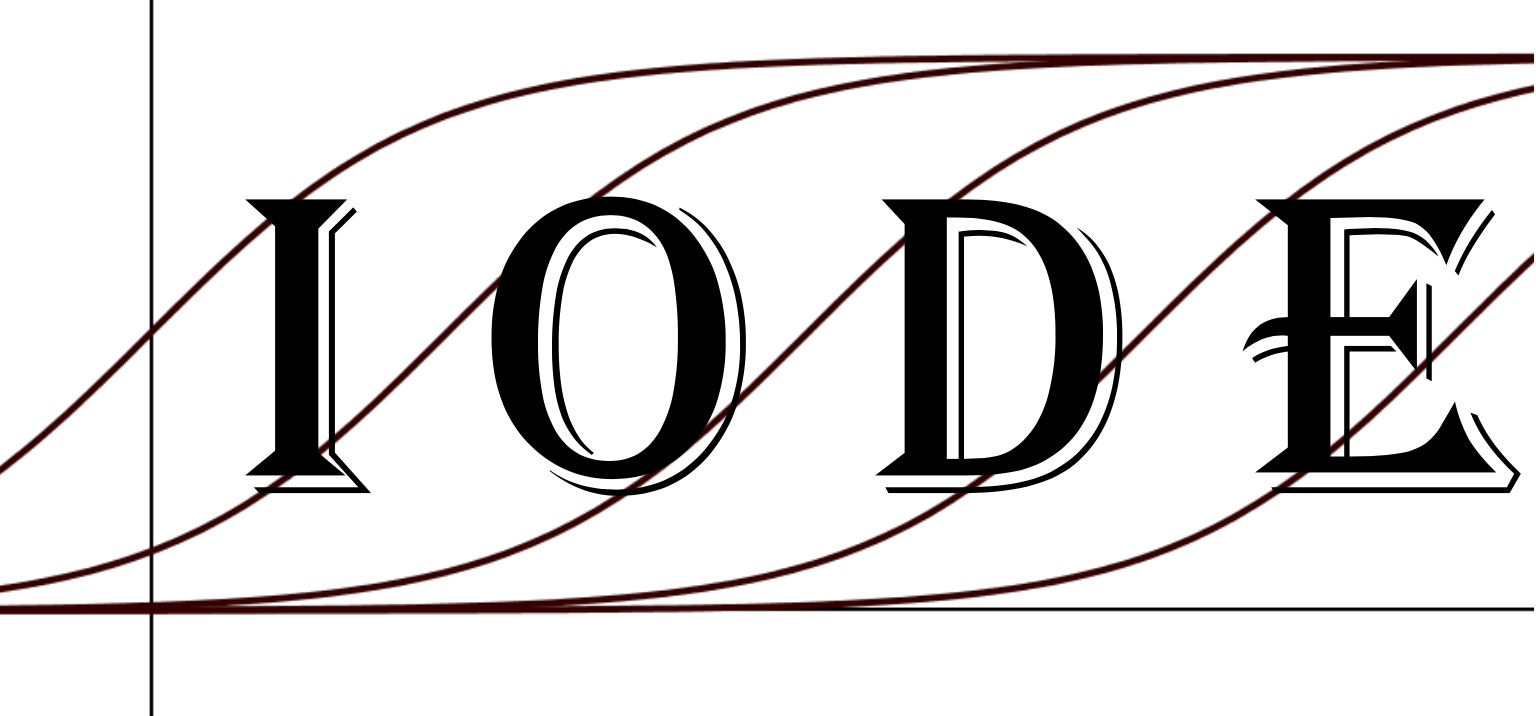
\includegraphics[width=1.25cm]{IODE-logo.png}}
\rfoot{\mypage}
\lfoot{}
\cfoot{}
\fancypagestyle{firstfooter}{\footskip = 50pt}
\renewcommand{\footrulewidth}{.4pt}
%%%%%%%%%%%%%%%%%%%%%%%%%%%
\vspace*{-20pt} \thispagestyle{firstfooter}
\pagebegin{Antiderivatives as Solutions}

\bbox
\begin{ex}
We can solve a differential equation of the form
\[ \frac{dy}{dt} = 6t^2\]
since the solution to the differential equation are all functions $y$ that have  $\frac{dy}{dt} = 6t^2$. Thus, $y$ must be an antiderivative of $6t^2$,
\[ y= \int \frac{dy}{dt} \ dt  = \int 6t^2 dt = 2t^3 + C.\]

\bi
\ii We say $y=2t^3+C$ is the \textbf{general solution} to the differential equation. The general solution gives all possible solutions to the original differential equation.
\ii If we are given additional information such as an \textbf{initial condition}  $y(t_1)=y_1$, then we get a unique solution.
\ei

For example, if we are given that $\frac{dy}{dt} = 6t^2$ and $y(2)=10$, first we find a general solution, and then we plug the initial condition into the  general solution and solve for the general constant $C$:
\[ y(2)=2(2)^3+C=16+C=10.\]
Thus, the solution will pass through the point $(2,10)$ only if $C=-6$. The solution to the \textbf{initial value problem (IVP)} is
\[ y=2t^3-6.\]
\end{ex}
\ebox

Differential equations of the form  $\frac{dP}{dt} = f(t)$ are a very special case since the derivative does not depend on the dependent variable. We have seen these differential equations are antiderivatives in disguise, and we can find a general solution by integrating both sides with respect to the independent variable.

\bb
\ii Can we apply the same method to solve an \textbf{autonomous} differential equation such as  $\frac{dy}{dt} = 0.2y$? Explain what looks wrong with each of the possible solution strategies below.
\bb
\ii $\dsty \int \frac{dy}{dt} \ dt = \int 0.2y \ dt$ \vspace{0.5in}
\ii $\dsty \int \frac{dy}{dt} \ dy = \int 0.2y \ dy$ \vspace{0.5in}
\ii $\dsty \int \frac{dy}{dt} \ dt = \int 0.2y \ dy$
\ee
\ee

\clearpage

\pagebegin{Finding the Exact Solution}

\bb[resume]
\item For a particular species of fish in a lake, the differential equation below models the rate of change of the fish population $P$ (measured in thousands of fish) $t$ years from now.
\[ \frac{dP}{dt} = 0.2P\]


\bb
\item Using the chain rule find a formula for $\frac{d}{dt} \left( \ln{P} \right)$, where $P$ is shorthand for $P(t)$. \label{05problem2partb}
\end{enumerate}
\vfill

%\clearpage

Next you will learn a technique for finding the exact solution using the result of the chain rule we identified in \ref{05problem2partb}. 

\begin{enumerate}[resume]
\item	 The following is a method to find the analytic solution to $\displaystyle\frac{dP}{dt}= 0.2P$. For now assume that $P > 0$. This assumption corresponds to the population growth context and it will make the algebra easier and hence the underlying idea clearer.  \label{05problem2partc}
 
\end{enumerate}

\begin{center} \renewcommand{\arraystretch}{1.5}
\newcolumntype{V}{>{\centering\arraybackslash} m{.5\linewidth} }
\begin{tabular}{|p{2in}|V|}
\hline

Divide both sides of \newline $\frac{dP}{dt}=0.2P$ by $P$ &
{} \\
{} & {} \\
\hline

Replace $\frac{1}{P}\frac{dP}{dt}$ with $\left[ \ln(P)\right]'$ & 
{} \\
{} & {} \\
\hline
	 
Write integrals with respect to $t$ on both sides & 
\\{} & {} \\ 
\hline
	 
Apply the Fundamental Theorem of Calculus to integrate both sides & 
\\{} & {} \\
\hline	 

Solve for $P$ (and remember that $P$ is actually a function, $P(t)$) & 
\\{} & {} \\
\hline

Show that $P$ can be written as $P(t) = ke^{0.2t}$ & 
\\{} & {} \\
{} & {} \\
\hline
\end{tabular} \end{center}

The end result, $\displaystyle P(t)=ke^{0.2t}$ is called the \textbf{general solution} because it represents all possible functions that satisfy the differential equation. We can use the general solution to find any \textbf{particular solution}, which is a solution that corresponds to a given \textbf{initial condition}.

\clearpage

\item	Use the same technique to find the general solution to $\displaystyle\frac{dy}{dt}=\frac{t}{3y^2}$. The first step is done for you. \label{05problem3}
\vs
$\displaystyle 3y^2\frac{dy}{dt}=t$
\vfill

%\clearpage

\item In practice, we often circumvent explicit use of the chain rule and instead use a shortcut to more efficiently find the general solution. The shortcut involves treating the derivative $\frac{dP}{dt}$ as a ratio and ``separating'' the $dP$ and $dt$. In the table below, follow the instructions to see how the shortcut works, using again the equation $\displaystyle\frac{dP}{dt} = 0.2P$. (See \href{http://kevinboone.net/separation_variables.html}{\underline{http://kevinboone.net/separation\textunderscore variables.html}}) for a nice explanation of the shortcut). \label{05problem4}
\vs

\begin{center}\renewcommand{\arraystretch}{1.5}
\newcolumntype{V}{>{\centering\arraybackslash} m{.5\linewidth} }
\begin{tabular}{|p{2.5in}|V|}
\hline
`Separate' the $dP$ from the $dt$ so that $dP$ and $P$ are on the same side. (If there are $t$'s in the equation they must go on the same side as $dt$.)
	  &
{} \\\hline

Integrate both sides of the equation (one side with respect to $P$, the other with respect to $t$)	  &
{} \\\hline

Continue as before to arrive at a solution of the form $P(t)=\underline{\hskip1cm}$	 	  &
{} \\
{} & {} \\
{} & {} \\
{} & {} \\
{} & {} \\
{} & {} \\
{} & {} \\
{} & {} \\ \hline
\end{tabular}
\end{center}

\item	Use the shortcut to find the general solution to  $\displaystyle \frac{dy}{dt}=\frac{t}{3y^2}$. \label{05problem5}
\vfill
\ee

\clearpage

A differential equation is called \textbf{separable} if it can be written in the form
\[ \frac{dy}{dx}=p(x,y)=f(x)g(y). \]
For example, the differential equation $\dsty \frac{dy}{dt}=\frac{t}{3y^2}$ is separable since it can be written as 
\[ \frac{dy}{dt}=(t)\left( \frac{1}{3y^2} \right).\]

\bb[resume]
\ii Decide whether the differential equation is separable.  If
so, separate it into the form $\dsty \frac{1}{g(y)} dy = f(x) dx$.

\bb
\ii $y' = 3x+y^2$ \vfill 
\ii $\displaystyle \frac{dy}{dt} = t^2y+ty$ \vfill
\ii $\displaystyle \frac{dz}{dw} = e^{z+w}$ \vfill
\ii $y'=\ln{(xy)}$ \vfill 
\ii $\displaystyle \frac{dy}{dx}-xy =0$ \vfill
\ee


\clearpage

\ii Solve the initial value problem. To solve an IVP one first must find the general solution and then use the initial condition to find the particular solution corresponding to the initial condition.

\bb
\ii $z' = \frac{qz}{z^2+1}$, $z(2)=1$ \vfill
%\ii $\dsty \frac{dx}{dt}= \frac{x\ln{x}}{t}$, $x(1)=6$ \bigskip

\ii $\dsty \frac{y'}{x}= \frac{\sin{(x^2)}}{y}$, $y(0)=3$  \vfill
\ee


\clearpage

\item Solve the following IVP:    
\[ \frac{dy}{dt}=\frac{t}{y}\hspace{0.5in} y(2)=-1\]
\vfill

\begin{enumerate}
\item	 For what values of $t$ is your solution valid? Why? \label{05problem6parta} 
\vskip1cm

\item Check to see that your {particular} solution ``fits'' the differential equation by substituting the solution and its derivative into the original differential equation. \label{05problem6partb} 
\vfill

\item	Use the GeoGebra applet, \href{https://ggbm.at/SbHk2n4H}{\underline{https://ggbm.at/SbHk2n4H}}, to check to see that your specific solution ``fits'' the differential equation by plotting the slope field and then plotting the graph of the solution on top of the slope field. Explain how this relates to Jerry's approach. \label{05problem6partc}

\vspace{-.25in}\hspace{-.75in}
\includegraphics[width=0.5in]{05/05IVPQR.png}
\vfill

\item Even though $\displaystyle\frac{dy}{dt}$ is undefined when $y=0$, the solution function can be defined such that $y(2)=0$.  What should the graph of this solution look like in the slope field? \label{05problem6partd} 
\vfill
\end{enumerate}

\end{enumerate}
